
\documentclass{beamer}
%\usepackage{beamerarticle}
\usepackage{fancyhdr}
\usepackage{amsmath, amscd}
%\usepackage{enumerate}
\usepackage{amsthm}
\usepackage{amssymb}
%\usepackage[pdftex]{graphicx}
\usepackage{verbatim}
\usepackage[all]{xy}
%\usepackage{hyperref}
%\usepackage{homework}
%\usepackage[top=1.5in, bottom=1in, left=1.25in, right=1.25in]{geometry}

\def\baselinestretch{1} % not quite double spaced


\input{gsDefns}

\mode<presentation>
{
  \usetheme{default}
  \usecolortheme[RGB={46,100,115}]{structure}
  \usecolortheme{crane}
  \usecolortheme{orchid}
  \usecolortheme{whale}
  \useoutertheme{infolines}
}


\usepackage[english]{babel}


\usepackage[latin1]{inputenc}


\usepackage{times}

\title[Creddit score]{Creddit score}


\author[Sisodia]{Gautam Sisodia} 

\subject{Talks}

\begin{document}

\begin{frame}
\titlepage

\end{frame}


\begin{frame}
\frametitle{The problem}

Online conversations can be frustrating

\pause

\begin{itemize}
\item misunderstandings
\pause
\item bad feelings
\pause
\item plus trolls
\end{itemize}

\pause

\hfil

Can I tell if the comment I'm thinking of posting will be helpful, or ignored, or trollish?

\pause

\hfil

Answer: a reddit comment score predictor

\end{frame}

\begin{frame}
\frametitle{Input/output}

\begin{figure}[h]
\centering
\makebox[\textwidth][c]{\includegraphics[width = 0.9\textwidth]{input_output}}
\end{figure}


\end{frame}

\begin{frame}
\frametitle{One interesting feature: the age of the comment}

\begin{figure}[h]
\centering
\makebox[\textwidth][c]{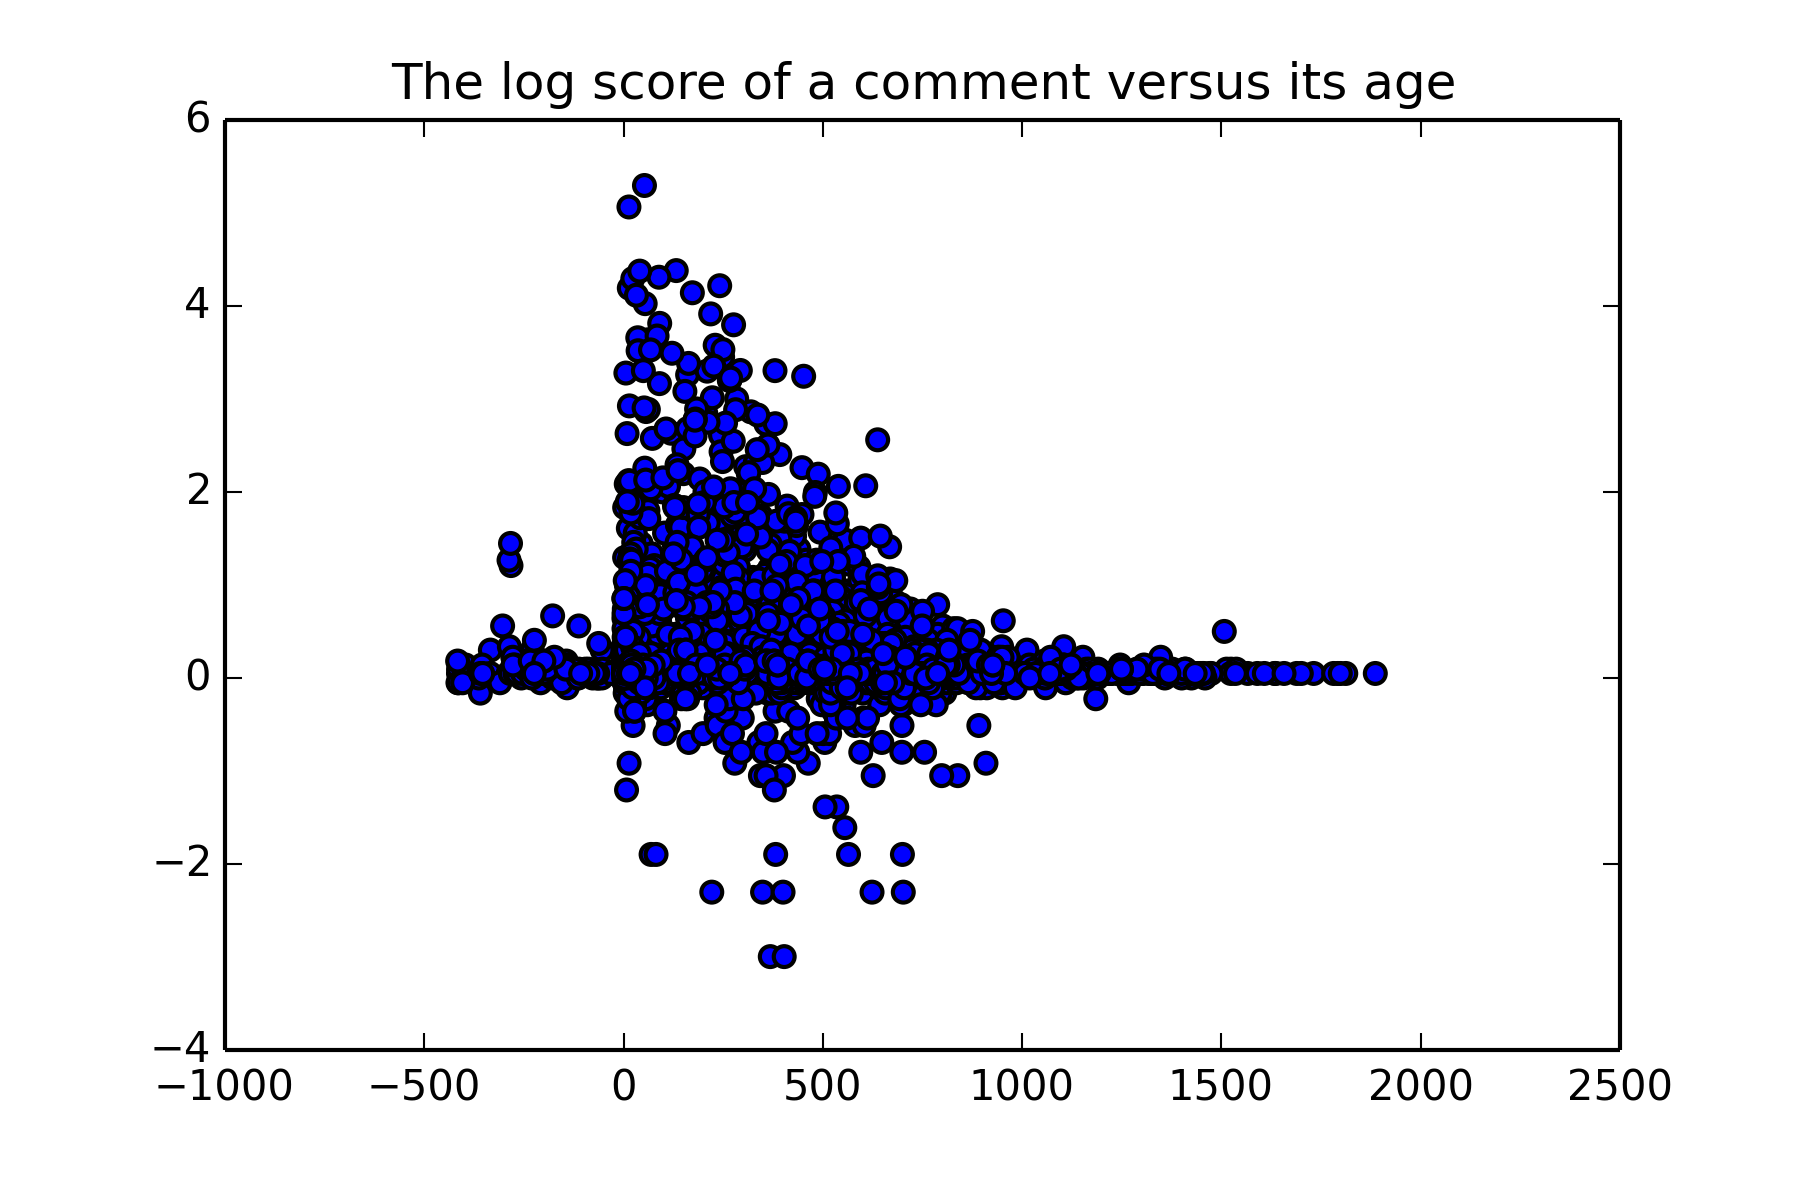
\includegraphics[width = \textwidth]{scoreVSage}}
\end{figure}


\end{frame}

\begin{frame}
\frametitle{Algorithm/analysis}

Features to extract:

\begin{itemize}
\item sentiment
\pause
\item relevance
\pause
\item length of comment
\pause
\item percent capitalization
\end{itemize}

\pause

Algorithm: 
\begin{itemize}
\item linear regression
\pause
\item make it classification (score $<$ 0, between 0-10, or $>$ 10) and decision tree
\end{itemize}

\end{frame}


\end{document}

